\documentclass[12pt]{article}
\usepackage{geometry}

%-----------------------------format.tex-----------------
\usepackage{amsmath,amssymb}
\usepackage{graphicx}
\usepackage{fancybox}
\usepackage{fancyhdr}
\usepackage{lastpage}
\usepackage{hyperref}
\hypersetup{
    unicode={true},pdfstartview={FitH},pdfborder={0 0 0},
    colorlinks,linkcolor=blue,citecolor=blue,hyperindex,plainpages=false,}
% style: page layout
\setlength{\headheight}{15pt}
\setlength{\headsep}{20pt}
\setlength{\footskip}{30pt}
\setlength{\voffset}{-5pt}
\setlength{\hoffset}{16pt}
\setlength{\oddsidemargin}{0pt}
\setlength{\evensidemargin}{\oddsidemargin}
\setlength{\marginparpush}{0pt}
\setlength{\marginparwidth}{0pt}
\addtolength{\textheight}{3\baselineskip}
\hypersetup{
	colorlinks=true,
	linkcolor=black
}
\newtheorem{definition}{{definition}}
\newcounter{numdefinition}
\renewenvironment{definition}[1]
{\noindent\stepcounter{numdefinition}
\slshape Definition \arabic{numdefinition} \textsf{#1 :}
\begin{quote}\small\itshape}
{\end{quote}}

\newcommand{\dd}{\ensuremath{\,\mathrm{d}}}
%===============================================================
\fancypagestyle{plain}%���¶���plain��ʽ,����summary sheet
{\fancyhf{}
\setlength{\headheight}{0pt}\setlength{\headsep}{0pt}
\setlength{\voffset}{-50pt}\setlength{\oddsidemargin}{0pt}}

\graphicspath{{pic/}}
%=========================����ҳü===============================
\pagestyle{fancy} 
\rhead{page\thepage\ of \pageref{LastPage}}
\chead{} \lhead{Team \footnotesize{\#} 201906177} \lfoot{}
\cfoot{\thepage}
\rfoot{}
\renewcommand{\headrulewidth}{0.4pt}

\begin{document}

%=========================summary sheet.tex========================

\thispagestyle{empty}
\begin{minipage}{0.3\textwidth}
%\begin{flushleft}
%For office use only\\
%   T1\ \rule{3cm}{0.5pt}\\
%   T2\ \rule{3cm}{0.5pt}\\
%   T3\ \rule{3cm}{0.5pt}\\
%   T4\ \rule{3cm}{0.5pt}\\
%\end{flushleft}
\end{minipage}\hspace{\fill}
\begin{minipage}{0.3\textwidth}
\centering
Team Control Number\\[5pt]
\fontsize{20pt}{\baselineskip}\selectfont  \textbf{201906177} \normalsize\\[10pt]
Problem Chosen\\[5pt]
\fontsize{18pt}{\baselineskip}\selectfont \textbf{A }\normalsize\\
\end{minipage}\hfill
\begin{minipage}{0.35\textwidth}
%\begin{flushright}
%\shortstack[l]{
%For office use only\\
%   F1\ \rule{3cm}{0.5pt}\\
%   F2\ \rule{3cm}{0.5pt}\\
%   F3\ \rule{3cm}{0.5pt}\\
%   F4\ \rule{3cm}{0.5pt}}
%\end{flushright}
\end{minipage}\vspace*{10pt}
\rule{\textwidth}{0.5pt}

\begin{center}
  \textbf{ShuWei Cup}
\end{center}
%\enlargethispage
\noindent
{\Large \textbf{Summary}}
\vspace{7pt}

%==========================abstract.tex================================
aaaaaaaaaaaaaaaaaaaaaaaaaaaaaaa

\textbf{keyword}: sweet spot; corked bat; coefficient of restitution;%xxx speed; finite element method; 
\newpage

%====================Ŀ¼ҳ========================================
\thispagestyle{empty}
\setcounter{page}{0}
{\begin{center}\Large \textbf{}\end{center}}
\tableofcontents                                                  %
\newpage                                                          %
%==================================================================

\newcommand{\vw}{\frac{v_i}{\omega_i}}

%=======================\input{introduction1}=======================

\section{Introduction}	
\subsection{Background}

\subsection{Work}

%============================\input{definitions1}===========
\section{Problem Analysis}
\paragraph{Analysis of question one}

Make reasonable predictions of the aging trend of China and the medical needs of the residents according to the data of residents' income, age structure of the population and the economic development level etc. in the relevant statistical analysis data of the National Bureau of Statistic. 
According to the relevant data from 2009 to 2018 in the National Bureau of statistics, the group first selects appropriate indicators and then establishes a grey prediction model to predict and analyze the population aging trend and residents' medical needs of the epidemic in 2009-2018. Then, through the Markov model, the data from 2009-2018 simulates the distribution of residual in each interval and calculates the expectation of the predicted residual in 2010-2019 Value. Finally, the prediction results and residual expectation are made to be different, and the inherent deviation of traditional grey prediction is corrected. Through the combination of the two models, the goal of scientific prediction of the future development of population aging and the trend of residents' medical needs is achieved. Its thought flow chart is shown in Figure ~\ref{lct}~ :


\paragraph{Analysis of question two}

\paragraph{Analysis of question three}
\paragraph{Analysis of question four}

\paragraph{Analysis of question five}
%=======================\input{Assumptions1}=====================================
	\section{Symbol and Assumptions}
\subsection{Symbol Description}
\begin{center}
\begin{tabular}{ll}
	\hline
	symbols&definitions\\
	\hline
	$v_i$& velocity of ball before collision\\
	$v_f$& velocity of ball after collision\\
	$V_f$& velocity of bat after collision\\
	$S$ & the shear modulus the bat\\
	$Y$ & Young��s modulus of the bat\\
	\hline
\end{tabular}
\end{center}


\subsection{Fundamental assumptions}
\begin{enumerate}
\item The bat is rigid, so there is no vibration in the bat(for the basic model).
\item The ball hit and rebound perpendicular to the bat and is in the plane of the swing.
\item The ball can be considered as a linear spring with friction.
\item The bat is a free object in collision,and both ends of the bat is completely free.
\item The vibration of the bat is harmonic(for augmented model).
\end{enumerate}

%=============================\input{ModelforCollision}==========================
\section{Establishment and solution of the model}

 \subsection{The model of Problem 1}
	\subsection{solution of the model 1}   
\begin{center}
\begin{figure}[htpb]
\centering
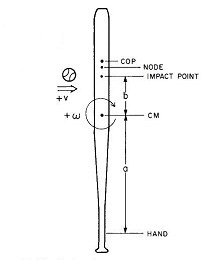
\includegraphics[scale=0.8]{locationofpoint}
\caption{location of point}\label{fig:locationofpoint}
\end{figure}
\end{center}

\begin{eqnarray}
m\cdot v_i=m\cdot v_f+M\cdot V_f \\
b\cdot m\cdot v_i+I\cdot \omega_i=b\cdot m\cdot v_f+I\cdot \omega_f\\
e_0\cdot (v_i-\omega_i\cdot b)=V_f+\omega_f\cdot b-v_f
\end{eqnarray}

\subsection{Conclusion}

\begin{center}
\begin{figure}[htpb]
\centering
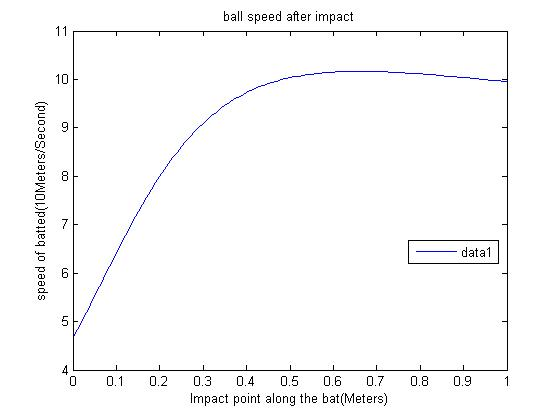
\includegraphics[scale=0.6]{firstwen}
\caption{final velocity $v_f$ varies by impact point location $b$}\label{fig:maximum}
\end{figure}
\end{center}
	  \subsection{The model of Problem 2}



\subsection{The model of Problem 3}



\subsection{The model of Problem 4}
%===========================  \section{Sensitivity Analysis}===============================
  \section{Sensitivity Analysis}

%====================================\input{StrengthsandWeaknesses}============================================
\section{Strengths and Weaknesses}

\subsection{Strengths}
\begin{enumerate}
\item Vibration of bat is taken into account so that the accuracy of the model can be fairly good.
\item Physical explanation is put forward besides the model for a better understanding of the collision process.
\item Figures are used for explanation of the problem,thus making it more intuitive and easier to understand.
\end{enumerate}

\subsection{Weaknesses}
\begin{enumerate}
\item The ball is actually nonlinear when deformation of the ball go beyond a certain limit.The approximation of linear model turned to be flawed when the force applied on the ball become very large.
\item Effective coefficient of restitution can not be calculated accurately.This affect the accuracy of the result of the model.
\end{enumerate}

\section{Conclusion}
%========================Bibtex
\newpage
	\nocite{*}		%??????????
%\bibliography{wenxian.bib}
%	%???????wenxian.bib?????
%	
\begin{thebibliography}{9}%??9
	\bibitem{bib:one}Saad Ahmed Javed,Sifeng Liu. Correction to: Predicting the research output/growth of selected countries: application of Even GM (1, 1) and NDGM models[J]. Scientometrics,2019,120(3).
	\bibitem{bib:2}???,???,???.?????????????????[J].??????,2018(15):74-75.	
	\bibitem{bib:3}Yawen Wang,Zhongzhou Shen,Yu Jiang. Analyzing maternal mortality rate in rural China by Grey-Markov model[J]. Medicine,2019,98(6).
	\bibitem{bib:4}Saad Ahmed Javed,Sifeng Liu. Correction to: Predicting the research output/growth of selected countries: application of Even GM (1, 1) and NDGM models[J]. Scientometrics,2019,120(3).
	\bibitem{bib:5}??,???,???.??????GM(1,N)-Markov???????[J].??????,2019(03):43-48.
	\bibitem{bib:6}???,???,???,???.??GM(1,1)?????????GM(1,1)????????????????[J].???????,2011,45(09):1075-1079.
	\bibitem{bib:7}Kate Childs,Christopher Davis,Mary Cannon,Sarah Montague,Ana Filipe,Lily Tong,Peter Simmonds,Donald Smith,Emma C. Thomson,Geoff Dusheiko,Kosh Agarwal. Suboptimal SVR rates in African patients with atypical Genotype 1 subtypes: implications for global elimination of Hepatitis C[J]. Journal of Hepatology,2019.
	\bibitem{bib:8}Yuyan Cao. Failure Prognosis for Electro-Mechanical Actuators Based on Improved SMO-SVR Method[A]. ?????????????????????????????????IEEE??????????.Proceedings of 2016 IEEE Chinese Guidance, Navigation and Control Conference (IEEE CGNCC2016)[C].2016:6.
\end{thebibliography}

\newpage
%??
%\appendix %%??

\end{document}
